\documentclass{article}
\PassOptionsToPackage{numbers,sort&compress}{natbib}
\usepackage[dblblindworkshop]{neurips_2026}
\usepackage[utf8]{inputenc}
\usepackage[T1]{fontenc}
\usepackage{amsmath,amssymb,booktabs,graphicx,microtype}
\usepackage[hidelinks]{hyperref}
\title{Persistent Data-Order Effects in Language Models:\\Dynamical Traces and Limits of Recovery Probes}
\workshoptitle{DynaFront 2: Dynamics at the Frontiers of Optimization, Sampling, and Games}
\author{Anonymous Authors}
\newcommand{\KL}{\operatorname{KL}}
\newcommand{\R}{\mathbb{R}}
\begin{document}
\maketitle
\begin{abstract}
Changing training-data order changes a model's optimization trajectory, but a persistent endpoint difference need not reveal when its direction stabilizes or whether it can be corrected. We study these distinctions using public Pythia-160M checkpoints trained on 300 billion tokens. At the final checkpoint, three correlated order-only pairs have symmetric KL divergence of 0.290--0.293 nats, approximately 3.8 times an adjacent-checkpoint drift reference and 95\% of the divergence of one joint initialization-and-order pair. These comparisons use a training-distribution shard; they hold late in training and do not isolate initialization effects. Functional divergence is already substantial while the raw endpoint-difference direction remains weakly aligned. Two subsequent probes fail their declared validity criteria: most parameter-block grafts degrade language modeling beyond a frozen loss band, and no tested Fisher estimator predicts all three local perturbations within 25\% relative error. We connect these observations to a fixed-subspace correction floor and delimit what remains unmeasured: functional recoverability and the cost of changing a completed training history.
\end{abstract}

\section{Introduction}
An optimization history is an ordered composition of update maps. Even with the same initial state and data multiset, changing the order can change the endpoint. A dynamical view asks how local order defects propagate through later updates, which aspects survive in the model's predictions, and which can be removed by a restricted correction. These are different questions: a large endpoint difference alone proves neither expensive correction nor irreversibility.

Public checkpoint suites make it possible to examine these distinctions without training new language models. Pythia provides trajectories across model sizes \citep{pythia}; PolyPythias varies initialization and data order \citep{polypythias}. We use their 160M-parameter runs as a controlled entry point into history dependence. Our contribution is a bounded empirical study of persistent order effects, the timing of their raw parameter direction, and the validity of two proposed recovery measurements. We do not present a successful large-scale transport operator or a general computational lower bound.

Local commutator criteria already address training-order selection \citep{rukhovich,sweeney}; our target is the persistent difference between completed histories. We separate direct measurements from recovery claims and retain failed measurement gates as outcomes. Section~2 states the dynamical framework and a restricted correction floor; Sections~3--4 report the checkpoint measurements and failed probes; Section~5 bounds their interpretation.

\newpage
\section{Dynamical framework and measurement design}
\paragraph{Transported order defects.}
Let $x$ include parameters and any optimizer state, and let $U_i$ be one update map. The adjacent-swap defect is
\begin{equation}
 \delta_{ij}(x)=U_j(U_i(x))-U_i(U_j(x)).
\end{equation}
For smooth SGD updates $U_i(x)=x-\eta g_i(x)$,
$\delta_{ij}(x)=\eta^2(Dg_j(x)g_i(x)-Dg_i(x)g_j(x))+O(\eta^3)$.
Thus the leading local defect is the established commutator term \citep{rukhovich,sweeney}. Stateful optimizers require the augmented state; the parameter-only SGD expansion cannot be applied unchanged to Adam.

Connect two update words by adjacent swaps. For swap $k$, let $z_k$ be the state after its first ordering, $z_k+\delta_k$ the state after its alternative, and $A_k$ their common remaining update composition. Their endpoint increment is exactly
\begin{equation}
 \Delta_k=A_k(z_k+\delta_k)-A_k(z_k),\qquad
 x_T^{(B)}-x_T^{(A)}=\sum_k\Delta_k.
\end{equation}
The second identity telescopes over the intermediate words. Differentiability gives the local approximation $\Delta_k\approx DA_k(z_k)\delta_k$: later dynamics can amplify, rotate, or cancel the defect. This identity supplies a framework, not an estimator validated here at 160M scale. Checkpoint differences below are direct observations, not reconstructed per-swap attributions.

\paragraph{A restricted correction floor.}
Let $\Delta\in\R^d$ be the parameter gap to a target, $S\subseteq\R^d$ a fixed linear subspace of allowed corrections, and $\Sigma\succeq0$ a fixed functional quadratic form. Define
\begin{equation}
 r_S(\Delta)=\min_{c\in S}\|\Sigma^{1/2}(\Delta-c)\|_2.
 \label{eq:floor}
\end{equation}
\textbf{Proposition.} If every cumulative correction lies in $S$, no such correction achieves quadratic-metric error less than $r_S(\Delta)$, at any compute budget.
\emph{Proof.} Every attainable residual is $\Delta-c$ for some $c\in S$ and hence has norm at least the minimum in Eq.~\eqref{eq:floor}. The minimum exists because $\Sigma^{1/2}S$ is a finite-dimensional linear subspace. A sequence of corrections in $S$ still sums to an element of $S$. $\square$

This elementary geometric floor depends on both the access class and the metric. It is exact for the stated quadratic model, not a global theorem about nonlinear output divergence. It gives no finite-budget scaling law and does not cover corrections whose reachable span changes with the state. A useful empirical application first requires a faithful $\Sigma$; Section~4 tests that prerequisite.

\paragraph{Models, metric, and controls.}
Write $m,d_1,d_2$ for the main Pythia-160M run and its two data-seed variants. They share an initialization. We analyze $P_1=(d_1,d_2)$, $P_2=(m,d_1)$, and $P_3=(m,d_2)$; these are three correlated pairs from three runs, not three independent replicates. The joint arm $J$ uses the two full-seed variants, changing initialization and order together. The endpoint is $T=143{,}000$ updates (300B training tokens).

For next-token distributions on a frozen shard $E$, our direct readout is
\begin{equation}
 D_E(a,b)=\frac{1}{2|E|}\sum_{x\in E}
 [\KL(p_a(\cdot|x)\|p_b(\cdot|x))+\KL(p_b(\cdot|x)\|p_a(\cdot|x))].
\end{equation}
The shard contains 48 non-overlapping 2,048-token blocks from \texttt{NeelNanda/pile-10k}, concatenated with EOS separators using the Pythia tokenizer: 98,304 prediction positions. It samples the training distribution, not a held-out generalization benchmark. Models run in evaluation mode with float32 forward passes and float64 accumulation. We compare 12 checkpoints from step 0 to $T$, omitting step 1 after an artifact audit found initialization copies. The candidate initialization-only arm failed continuity checks and was excluded before the amended comparison. Consequently, $D_E(J)-D_E(P_i)$ cannot identify an initialization main effect.

\newpage
\section{Persistent output differences, later directional alignment}
\begin{figure}[h]
\centering
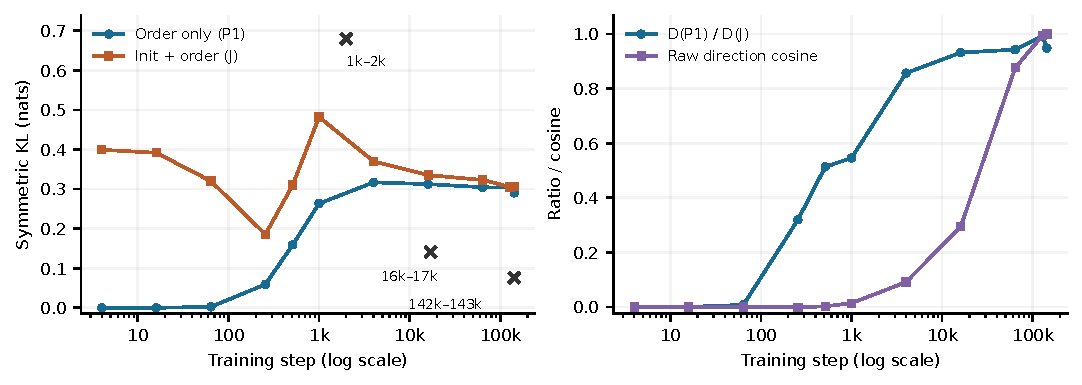
\includegraphics[width=\linewidth]{dynamics.pdf}
\caption{Recorded checkpoint measurements. Left: output divergence for one order-only pair and the joint pair; crosses are same-run drift over the labeled checkpoint windows, not statistical error bars. Right: the order/joint divergence ratio and raw endpoint-direction cosine for $P_1$. The quantities measure different objects; proximity of their numerical values has no metric interpretation. Lines connect the measured grid only.}
\label{fig:dynamics}
\end{figure}

\paragraph{Late-training order effects persist.}
Table~\ref{tab:endpoint} reports the endpoint measurements. The same-run drift reference is $D_E(d_{1,142000},d_{1,143000})=0.076275$; the 160M--410M comparison is 0.460360. Each order-only pair lies between these references. The order-only maximum/minimum ratio is 1.009, below the predeclared threshold of 2.0. The approximately 1\% agreement is descriptive; it is not a confidence interval or an independently replicated population estimate.

\begin{table}[h]
\centering
\caption{Final-checkpoint divergence on the frozen training-distribution shard. All three order-only pairs share one initialization; each run occurs twice. Ratios share the same single joint-pair denominator.}
\label{tab:endpoint}
\begin{tabular}{lrrr}
\toprule
Pair & $D_E$ (nats) & $D_E/D_E(J)$ & $D_E$/drift reference\\
\midrule
$P_1$: data-seed1 / data-seed2 & 0.290461 & 0.9489 & 3.81\\
$P_2$: main / data-seed1 & 0.290638 & 0.9494 & 3.81\\
$P_3$: main / data-seed2 & 0.293055 & 0.9573 & 3.84\\
$J$: full-seed1 / full-seed2 & 0.306112 & 1.0000 & 4.01\\
\bottomrule
\end{tabular}
\end{table}

The adjacent-checkpoint ``floor'' measures training drift, not numerical noise or a statistical detection limit. It depends strongly on time and the chosen 1,000-update window: its value is 0.680225 at steps 1,000--2,000 and 0.140831 at 16,000--17,000. Early pair values therefore do not establish separation from drift. The approximately 3.8-fold comparison is specifically a late-training result. The amended experiment tested an order-only persistence criterion weaker than the original two-arm criterion; the missing initialization-only comparison remains untested.

\paragraph{Magnitude and direction have different timing.}
For $P_1$, define $\Delta_t=\theta_{d_2,t}-\theta_{d_1,t}$ and $C_t=\langle\Delta_t,\Delta_T\rangle/(\|\Delta_t\|_2\|\Delta_T\|_2)$. At step 16,000, $D_E(P_1)/D_E(J)=0.932$, but $C_t=0.294$; at 64,000 these values are 0.943 and 0.877. The first sampled $C_t\geq0.9$ occurs at 128,000. The ratio is not monotone: it decreases from 0.993 at 128,000 to 0.949 at $T$.

The other correlated pairs have step-16,000 cosines 0.441 and 0.466 and cross 0.9 at 64,000. Thus the qualitative dissociation appears in all three pairs, with pair-dependent timing. Early directions are storage-quantization limited, and $C_T=1$ is an identity; nearby endpoints also correlate mechanically. These observations do not determine when a \emph{functional} direction locks in, nor when individual order defects were created. A stable scalar divergence need not imply a stable direction in output space.

\newpage
\section{Two recovery probes fail their validity gates}
\paragraph{Parameter-type grafts leave the allowed loss region.}
At $T$, we form hybrids by moving one parameter-type block of $d_1$ toward the corresponding block of $d_2$: $\theta_h=\theta_{d_1}+\alpha M_b(\theta_{d_2}-\theta_{d_1})$, with mask $M_b$. The frozen validity rule rejects a hybrid when its token cross-entropy exceeds the worse parent's loss by 0.5 nats, giving a threshold of 3.001560. The instrument checks passed, including reproduction of the recorded parent divergence to relative error $1.4\times10^{-10}$.

Seven of eight complete block swaps are invalid. Across evaluated interpolation cells, the loss band rejects 23 of 35. Attention QKV, carrying 87\% of the squared parameter gap, is invalid at every tested nonzero interpolation strength. Only the internal LayerNorm block remains valid through a complete swap; even that hybrid is degraded and far from both parents. The frozen abort rule stops the remaining control sequence. The formal outcome is inconclusive for spatial recoverability: these hybrids establish the failure of this graft class at the tested strengths, not a proof that the order trace cannot be edited.

\paragraph{Local Fisher metrics do not certify.}
To attempt Eq.~\eqref{eq:floor} without cross-model grafts, we test $D_E(\theta,\theta+v)\approx v^\top\Sigma_Ev$, with $\Sigma_E=\tfrac12\widehat F$. For the true predictive Fisher, this is the local quadratic approximation to the half-sum KL convention above. It is not generally the observed-label loss Hessian. The empirical Fisher and predictive Fisher are distinct objects \citep{kunstner}; replacing one by the other needs validation.

The frozen gate requires relative prediction error at most 0.25 on all three scaled probe directions: random, the last two checkpoints' update, and the endpoint order gap. Cross-entropy increases are 0.0050, 0.0337, and 0.0087 nats, respectively. Table~\ref{tab:fisher} reports the relative errors. No family passes; the planned projection ladder and Fisher-weighted direction timing are therefore unrun.

\begin{table}[h]
\centering
\caption{Local-metric certification on one endpoint pair. Each entry must be $\leq0.25$; the predictive-Fisher diagonal uses Monte Carlo sampling. A full empirical-Fisher diagnostic also fails all three probes.}
\label{tab:fisher}
\begin{tabular}{lrrrr}
\toprule
Estimator & Random & Update & Order gap & Passed\\
\midrule
Diagonal empirical Fisher & 1.11 & 0.77 & 0.47 & 0/3\\
Per-tensor empirical Gram & 1.90 & 0.61 & 1.31 & 0/3\\
Diagonal predictive Fisher & 0.524 & 0.811 & 0.126 & 1/3\\
\bottomrule
\end{tabular}
\end{table}

The predictive diagonal is accurate to 13\% along the endpoint gap, yet underpredicts the update-direction KL by about 5.3 times. This direction-dependent failure is consistent with missing cross-parameter curvature. The failure pattern repeats across independent Fisher builds, while the direct divergence readout reproduces to relative error $1.42\times10^{-10}$. Small loss changes alone do not certify the asymptotic quadratic regime or uniquely identify the error source; finite perturbations and estimator sampling remain limitations. No tolerance was relaxed after seeing these results.

\section{Discussion and limitations}
Order sensitivity is established prior work; early-training instability and mode connectivity already motivate studying timing \citep{frankle}. Our extension is a direct output-divergence comparison across completed language-model histories, paired with a distinction between divergence magnitude and raw direction and explicit failures of recovery probes. The fixed-subspace result is elementary and conditional: no calibrated functional correction floor has been measured here.

The evidence covers one model size, one shared initialization for the order-only runs, a single joint pair, and one training-distribution shard. There are no independent-seed error bars, downstream generalization results, or initialization-only control. These data cannot partition the remaining joint divergence into initialization and initialization--order interaction. Neither the failed grafts nor the failed metric establish universal irreversibility. The next useful experiment is certification of a metric carrying cross-parameter structure, with new probe criteria fixed before recovery measurements; low-rank metrics must also account for directions outside their represented subspace. Persistent order dependence is measurable here; cheap history correction remains open.

\clearpage
\begin{thebibliography}{9}
\bibitem{pythia} Stella Biderman et al. Pythia: A suite for analyzing large language models across training and scaling. \emph{ICML}, 2023. \url{https://arxiv.org/abs/2304.01373}.
\bibitem{polypythias} Oskar van der Wal, Pietro Lesci, Max Muller-Eberstein, Naomi Saphra, Hailey Schoelkopf, Willem Zuidema, and Stella Biderman. PolyPythias: Stability and outliers across fifty language model pre-training runs. \emph{ICLR}, 2025. \url{https://arxiv.org/abs/2503.09543}.
\bibitem{kunstner} Frederik Kunstner, Lukas Balles, and Philipp Hennig. Limitations of the empirical Fisher approximation for natural gradient descent. \emph{NeurIPS}, 2019. \url{https://arxiv.org/abs/1905.12558}.
\bibitem{frankle} Jonathan Frankle, Gintare Karolina Dziugaite, Daniel M. Roy, and Michael Carbin. Linear mode connectivity and the lottery ticket hypothesis. \emph{ICML}, 2020. \url{https://arxiv.org/abs/1912.05671}.
\bibitem{rukhovich} Alexey Rukhovich, Alexander Podolskiy, and Irina Piontkovskaya. Commute your domains: Trajectory optimality criterion for multi-domain learning. \emph{arXiv:2501.15556}, 2025. \url{https://arxiv.org/abs/2501.15556}.
\bibitem{sweeney} John Sweeney. The geometry of sequential learning: Lie-bracket prediction of transfer order. \emph{ICML}, 2026. \url{https://arxiv.org/abs/2606.24993}.
\end{thebibliography}
\end{document}
